\documentclass[a4paper,11pt]{article}
    \usepackage[utf8]{inputenc}
    \usepackage[italian]{babel}
    \usepackage[maxbibnames=99,backend=bibtex]{biblatex}
    \usepackage{hyperref}
    \usepackage{listings}
    \usepackage{color}
    \usepackage{graphicx}
    \usepackage{bigints}
    \usepackage{relsize}
    \usepackage{titling}
    \usepackage{fancyhdr}
    \usepackage{lipsum} 
    \addbibresource{ref.bib}
    \graphicspath{ {images/} }

    \lstset { %
        language=C++,
        frame=tb, 
        backgroundcolor=\color{lightgray}, 
        basicstyle=\footnotesize,
        numbers=left, 
        tabsize=4, 
        breaklines=true,
    }

    \definecolor{lightgray}{rgb}{.9,.9,.9}
    \definecolor{darkgray}{rgb}{.4,.4,.4}
    \definecolor{purple}{rgb}{0.65, 0.12, 0.82}

    \lstset{frame=tb,
        language=C++,
        breaklines=true,
        showstringspaces=false,
        columns=flexible,
        numbers=none,
        commentstyle=\color{dkgreen},
        stringstyle=\color{mauve},
        tabsize=3
    }
    
    \author{
        \rule{0in}{0pt}\textbf{\Large Candidato} \\
        \rule{0in}{0pt}Coccomini Davide \\
        \and
        \rule{1.5in}{0pt}\textbf{\Large Relatori}\\
        \rule{1.5in}{0pt}Pistolesi Francesco\\
        \rule{1.5in}{0pt}Lazzerini Beatrice \\
    }


    \pretitle{%
    \begin{center}
        \LARGE
        
\includegraphics[scale=0.4]{logo}\\[\bigskipamount]
    }
    \posttitle{\end{center}}
    \title{\textbf{UNIVERSITÀ DEGLI STUDI DI PISA} \\[0.4in]
    Scuola di Ingegneria \\
    Dipartimento di Ingegneria dell’Informazione \\
    A.A. 2018/2019\\[0.7in]
    Sviluppo di una rete neurale per il riconoscimento delle differenze percettive su un set di immagini alla ricerca della minima qualità necessaria per l'individuazione\\[0.8in]}
    \date{}
    
    \definecolor{mygreen}{rgb}{0,0.6,0}
    
    \lstset{  
        numbers=left,
        numbersep=5pt,
        commentstyle=\color{mygreen},
        keywordstyle=\color{blue}\ttfamily,
        stringstyle=\color{red}\ttfamily  
    }
    
    \hypersetup{colorlinks=true, linktoc=all,  linkcolor=black,citecolor=black}
    \newpage
    \begin{document}
    \pagestyle{fancy}
    \fancyhead{} 
    \renewcommand{\headrulewidth}{0pt}
    \fancyfoot{}
    \fancyfoot[LE,RO]{\thepage}    
    \fancyfoot[RE,LO]{Davide Coccomini - Università di Pisa 2018/2019} 
    \renewcommand{\footrulewidth}{0.4pt}
    \maketitle
    \newpage
        \tableofcontents
        \newpage
        \section{Introduzione}
        L'individuazione delle differenze percettive tra due o più immagini è uno dei grandi problemi dell'industria della colorimetria moderna che ha la necessità di emulare il 
        comportamento umano nella percezione dei colori. È infatti spesso necessario riprodurre un materiale o un tessuto partendo da un originale, nel tentativo di emularlo il più fedelmente possibile. 
        Per fare ciò, sono stati realizzati macchinari in grado di acquisire immagini ad alta definizione dei soggetti originali e di quelli riprodotti così da poterli confrontare attraverso indici matematici più o meno precisi (ad esempio SSIM) 
        nel tentativo di identificare eventuali differenze percettive. Ovviamente, sia per l'acquisizione che per il confronto tra immagini ad alta definizione, sono necessari tempi e costi non indifferenti che sarebbero abbattuti se questi processi potessero avvenire a risoluzioni più basse.
        Lo scopo di questa ricerca è quindi quello di realizzare una rete neurale che sia in grado di identificare le differenze tra le immagini e sfruttarla per capire qual è la minima risoluzione e qualità che le immagini devono possedere affinché queste differenze siano individuabili.
    
        \newpage
        \section{Colorimetria}
        La colorimetria è la disciplina che si occupa di normalizzare la misurazione del colore attraverso lo studio dei modelli di colore.
        \subsection{Lo spettro visibile}
        Tutte le colorazioni percepite dall’occhio umano compongono lo “spettro del visibile” che si trova nella parte centrale dello spettro ottico, il quale
        comprende anche i raggi infrarossi e quelli ultravioletti. 
        La colorimetria utilizza la percentuale della luce incidente che è stata riflessa compresa
        nell'intervallo del visibile (400-700 nm) per descrivere il colore dell'oggetto. Ciascun oggetto
        colorato viene pertanto definito da una curva di riflettanza, similmente alle impronte digitali
        nell’uomo. 
        \begin{figure}[h]
            \centering
            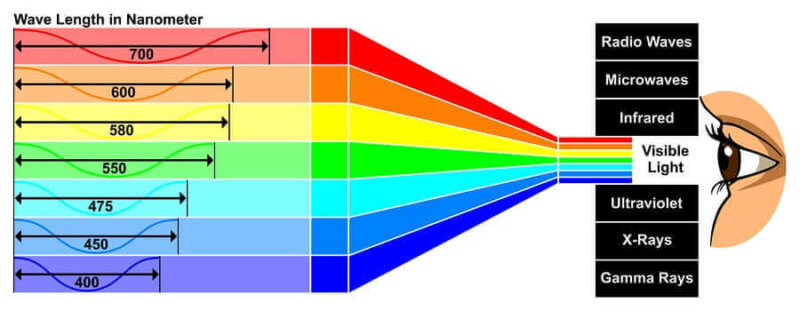
\includegraphics[scale=0.45]{colorimetria3}
            \caption{"Lo spettro visibile"}
        \end{figure}
        \newpage
        \subsubsection{Percezione del colore}
        Il colore nasce dalla luce. La luce che colpisce un oggetto viene parzialmente assorbita a
        seconda del materiale che lo compone. La parte non assorbita viene riflessa e trasmessa ai recettori cromatici
        all’interno dell’occhio umano. Questi ultimi trasformano la luce assorbita in impulsi che
        percorrono le vie nervose fino a raggiungere il cervello, dove vengono interpretati: nasce così
        un’impressione cromatica. Dal punto di vista prettamente biologico il colore si genera pertanto
        nell’occhio dell’osservatore e costituisce un’impressione sensoriale.
        Proprio perché nella percezione del colore vengono coinvolte componenti biologiche, ciascun individuo "percepisce" il colore in modo
        differente. Tale fenomeno può essere ricondotto sia al fatto che non esistono mai due occhi
        uguali tra loro sia al fatto che l’interpretazione del colore varia da individuo ad individuo.
        Perfino la stessa persona può percepire differentemente il colore in momenti diversi ed in base
        allo stato d’animo. È quindi molto complesso definire in maniera oggettiva un colore.

        \begin{figure}[h]
            \centering
            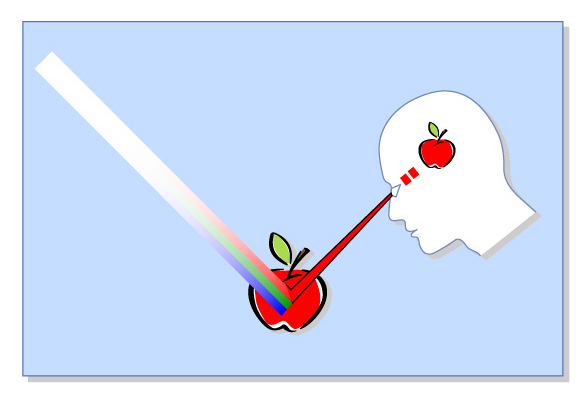
\includegraphics[scale=0.8]{colorimetria1}
            \caption{"Percezione del colore"}
        \end{figure}
        \newpage
        \subsection{Spazio colore}
        Gli spazi colore sono schemi di rappresentazione dei colori. Ognuno di essi si basa su alcuni parametri
        e facendoli variare riesce a rappresentare un numero più o meno grande di colori. Esistono numerosi spazi colore
        che, in base alle loro peculiarità, si prestano meglio ad uno specifico utilizzo piuttosto che ad un altro.
       
        \subsubsection{Modello CIE XYZ}
        Il modello CIE XYZ rappresenta tutti i colori caratterizzati da tre parametri: luminosità, tinta e purezza, rappresentati attraverso un solido. 
        Del solido viene solitamente rappresentata soltanto la sezione secondo il piano XY, in cui X ed Y indicano la cromaticità (tinta e purezza) mentre la luminosità non viene rappresentata.
        \begin{figure}[h]
            \centering
            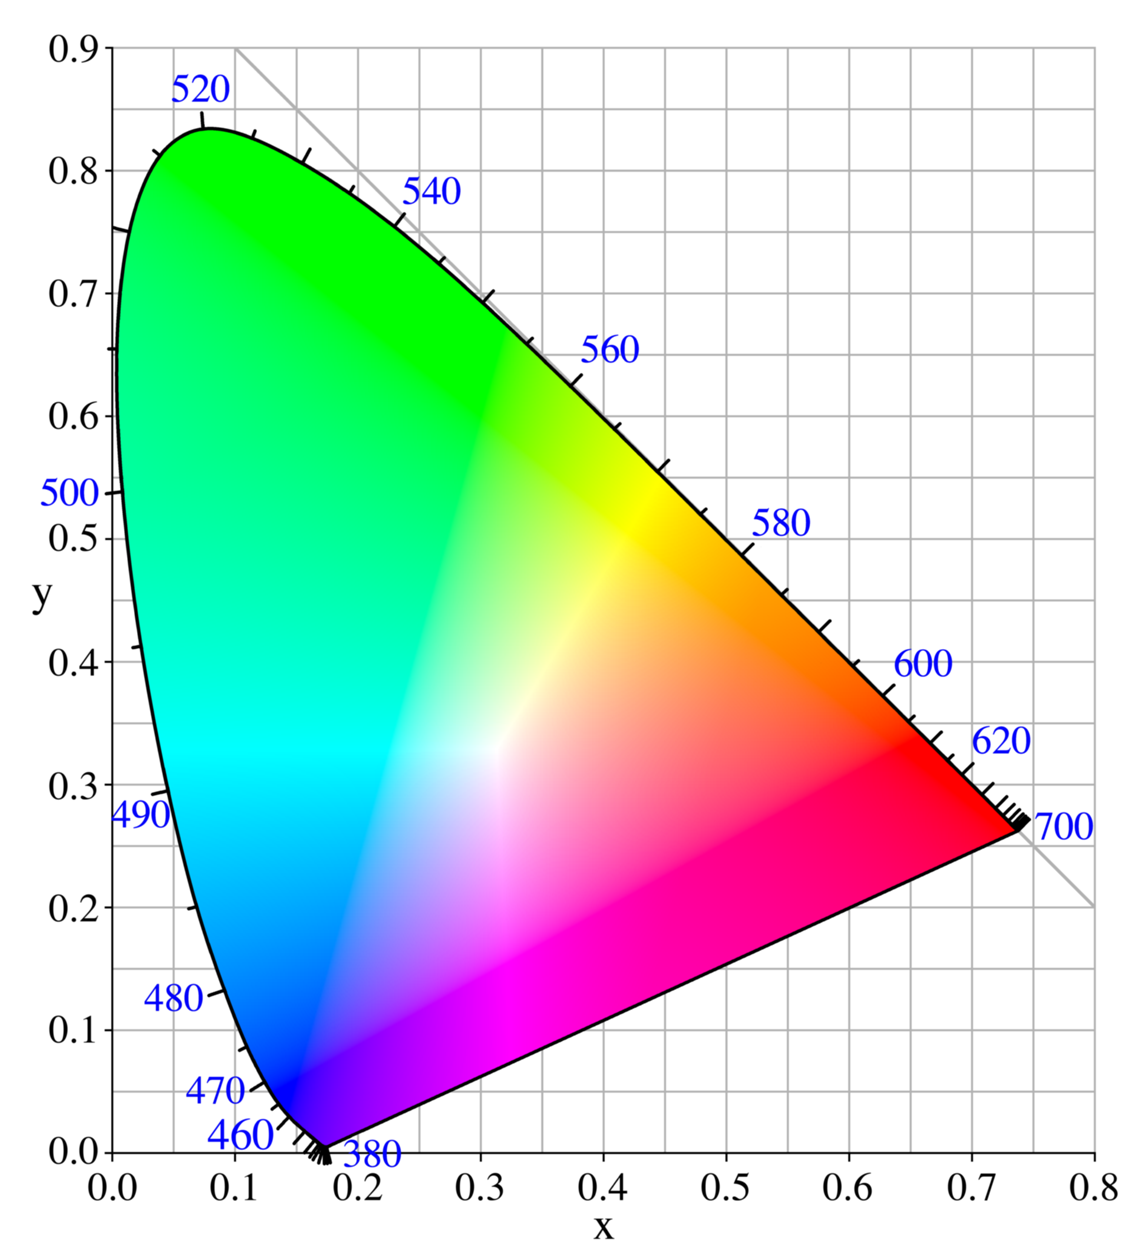
\includegraphics[scale=0.2]{CIEXYZ.png}
            \caption{"Spazio colore CIE XYZ"}
        \end{figure}
        \\Questo spazio colore si basa sui valori di tristimolo, cioè dei parametri che definiscono il modo in cui l'essere umano percepisce i colori. 
        I valori tristimolo di un colore con una distribuzione di potenza spettrale $I(\lambda)$  sono date in termini di un osservatore standard da:
        \\[0.2in]
            $\textbf{X}=\bigint_0^\infty I(\lambda)\,\overline{x}(\lambda)\,d\lambda$;
            $\textbf{Y}=\bigint_0^\infty I(\lambda)\,\overline{y}(\lambda)\,d\lambda$;
            $\textbf{Z}=\bigint_0^\infty I(\lambda)\,\overline{z}(\lambda)\,d\lambda$;
      
        
    
        \newpage

        \subsubsection{Modello CIE L*a*b*}
        Il modello CIE L*a*b*, è un'evoluzione del modello CIE XYZ. È un modello tridimensionale che si sviluppa lungo tre assi ortogonali. Due assi sul piano orizzontale riguardano la cromaticità: l'asse \textbf{a} si estende nel verde (-a) al rosso (+a)
        e l'asse \textbf{b} dal blu (-b) al giallo (+b); un asse verticale riguarda la luminosità o luminanza \textbf{L} che diminuisce dal basso verso l'alto.
        Questo particolare spazio colore include tutti i colori percepibili e quindi anche tutto il gamut degli spazi RGB e CMYK ed è indipendente dal dispositivo che li rappresenta.
        Essendo quindi molto più simile al modo in cui l'essere umano riesce a percepire i colori, questo spazio colore si presta particolarmente bene quando si devono individuare le differenze percettive all'interno di più immagini.

    
        \begin{figure}[h]
            \centering
            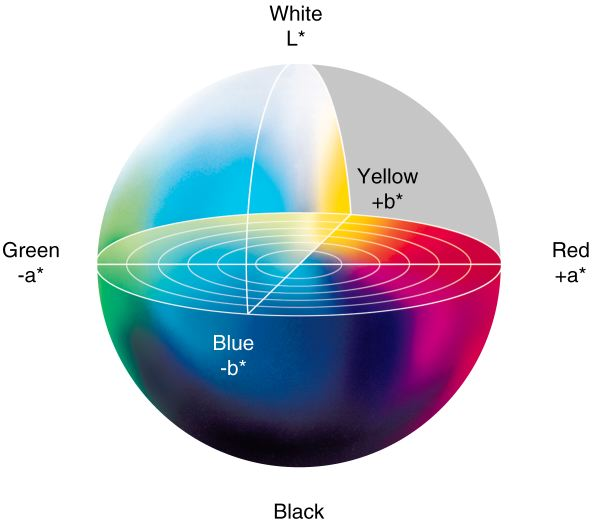
\includegraphics[scale=0.6]{CIELAB.jpg}
            \caption{"Spazio colore CIE L*a*b*"}
        \end{figure}

    \newpage
    \subsection{Risoluzione e compressione}
    La risoluzione di un'immagine corrisponde al numero di pixel per pollice che contiene, indicata con il termine in DPI (punti per pollice). 
    Un maggior numero di dpi si traduce in una maggiore quantità di informazioni e quindi in una migliore qualità dell'immagine. 
    Ovviamente, maggiore è il numero di informazioni che un'immagine contiene, maggiore sarà il peso del file. 
    Per questa ragione sono state sviluppate alcune tecniche di compressione tra cui quella JPEG. Questa tecnica stabilisce due metodi di compressione di base,
    uno basato sull'uso della trasformata discreta del coseno, con compressione di tipo "lossy" e cioè con perdita di informazione, e l'altro sull'uso di un metodo predittivo
    con compressione di tipo lossless, cioè senza perdita di informazione. La perdita di informazioni durante la compressione può compromettere drasticamente la qualità dell'immagine.
    \begin{figure}[h]
        \centering
        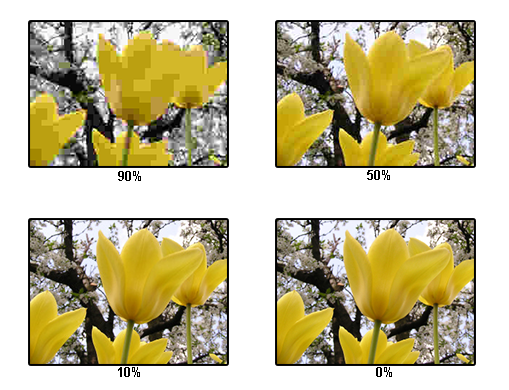
\includegraphics[scale=0.7]{jpeg.png}
        \caption{"Esempio di compressione JPEG"}
    \end{figure}
   
    \newpage
    \section {Reti Neurali}
    \subsection {Reti neurali e cervello umano}
    Le reti neurali artificiali sono nate per emulare attività tipiche del
    cervello umano. Risultano quindi molto utili per risolvere problemi di riconoscimento delle immagini o del linguaggio umano.
    Per riuscire ad emulare questi comportamenti ci si è quindi ispirati al funzionamento del cervello umano.
    Nel sistema nervoso esistono miliardi di neuroni. Un
    neurone è formato da un corpo cellulare e da molti prolungamenti
    ramificati, detti dendriti, attraverso i quali il neurone riceve segnali
    elettrici da altri neuroni. Ogni neurone ha anche un prolungamento
    filamentoso chiamato assone. All’estremità l’assone si ramifica formando terminali
    attraverso i quali i segnali elettrici vengono trasmessi ad altre cellule.
    Tra un terminale di un assone e la cellula ricevente esiste uno spazio. I segnali superano questo spazio per
    mezzo di sostanze chimiche dette neurotrasmettitori. Il punto di
    connessione tra terminale e dendrite è detto sinapsi. 
    Un neurone si “attiva”, cioè trasmette un impulso elettrico lungo il suo
    assone quando si verifica una differenza di potenziale elettrico tra l’interno
    e l’esterno della cellula. L’impulso elettrico provoca la liberazione di un
    neurotrasmettitore dai terminali dell’assone, che a loro volta possono influenzare altri neuroni. 
        
    \begin{figure}[h]
        \centering
        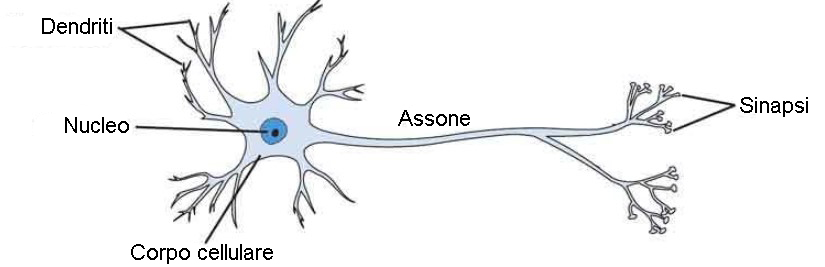
\includegraphics[scale=0.7]{cervello.jpg}
        \caption{"Neurone biologico"}
    \end{figure}

    \subsubsection{Dal neurone biologico a quello artificiale}
    
    Per riprodurre artificialmente il cervello umano occorre realizzare
    una rete di elementi molto semplici in grado di imparare e generalizzare.
    Tipicamente, il neurone artificiale ha molti ingressi ed una sola uscita.
    Per determinate la conducibilità e quindi l'importanza del canale di ingresso, ogni neurone ha associato un peso. 
    L’attivazione del neurone è una funzione della somma pesata degli ingressi.\\[1in]
    Il metodo più usato per addestrare una rete neurale consiste nel presentare
    in ingresso alla rete un insieme di esempi (training set). 
    La risposta fornita dalla rete per ogni esempio viene confrontata con la risposta desiderata, si
    valuta la differenza (errore) fra le due e, in base a tale differenza, si
    aggiustano i pesi cercando di ottenere il risultato desiderato.
    \begin{figure}[h]
        \centering
        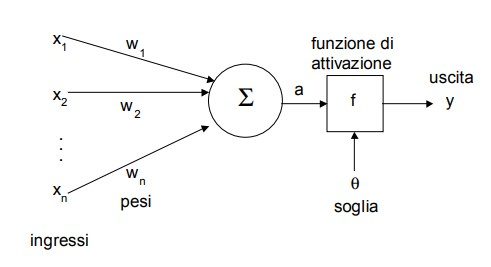
\includegraphics{neurone.jpg}
        \caption{"Modello di neurone"}
    \end{figure}
    \\Abbiamo $n$ canali di ingresso $x_1, …, x_n$, a ciascuno dei quali è associato un peso. 
    I pesi $w_i$ sono numeri reali che riproducono le sinapsi. Se $w_i > 0$, il canale è detto eccitatorio, se $w_i < 0$, il canale è inibitorio. 
    Il valore assoluto di un peso rappresenta la forza della connessione. 
    L’uscita, cioè il segnale con cui il neurone trasmette la sua attività
    all’esterno, è calcolata applicando la funzione di attivazione alla somma
    pesata degli ingressi:
    
    $$y = f(\sum_{i=1}^{n}w_i x_i)$$

    \subsection{Perceptron}
    Un perceptron è una rete neurale ad un singolo livello che si dimostra molto utile nei problemi di classificazione.
    In generale è composto da una serie $x_1, ..., x_n$ di inputs a cui sono associati dei pesi $w_1, ..., w_n$. 
    Vi è poi una funzione che si occupa di sommare i prodotti dei valori di input e dei rispettivi pesi. 
    Il risultato passa infine per una funzione di attivazione che genera l'output.

    \newpage
    \subsubsection{Addestramento del perceptron}
    Per addestrare un perceptron bisogna realizzare un training set adeguato per il problema che si vuole risolvere. 
    Dopo aver predisposto il dataset è necessario seguire i seguenti passi:
    \begin{enumerate}
        \item si inizializzano i pesi $w_i$ con valori casuali;
        \item si presenta alla rete un ingresso $x_k$ insieme al valore $t_k$ desiderato in uscita;
        \item si calcola la risposta $y_k$ della rete e si aggiornano i pesi mediante la delta rule;
        \item si ripete il ciclo dal passo 2, finché la risposta della rete non risulti soddisfacente.
    \end{enumerate}

    In particolare la delta rule è una regola usata per aggiustare i valori dei pesi di un neurone andando alla ricerca di quelli più adeguati.
    Dati $t$ ed $y$, rispettivamente, l'uscita desiderata e l'uscita neurale, l'errore $\delta$ è dato da:
    $$ \delta = t-y $$
    Fissato un numero reale $\eta$ compreso tra 0 e 1 detto learning rate, la delta rule stabilisce che la variazione del generico peso $\Delta w_i$ è:
    $$ \Delta w_i = \eta \delta x_i $$

    Dopo l’addestramento la rete viene testata controllandone il comportamento su un insieme di dati, detto test set, non utilizzati durante la fase di training. La fase di test ha quindi lo scopo 
    di valutare la capacità di generalizzazione della rete neurale.

  
    \newpage

    \section{Svolgimento}

    \subsection{Creazione del dataset}
    Per poter realizzare la rete è necessario creare un dataset significativo affinché questa possa essere addestrata e testata. 
    Per fare ciò sono state prese in considerazione 40 immagini ad una risoluzione di 4K sulle quali sono state successivamente fatte delle elaborazioni.
    \begin{figure}[h]
        \centering
        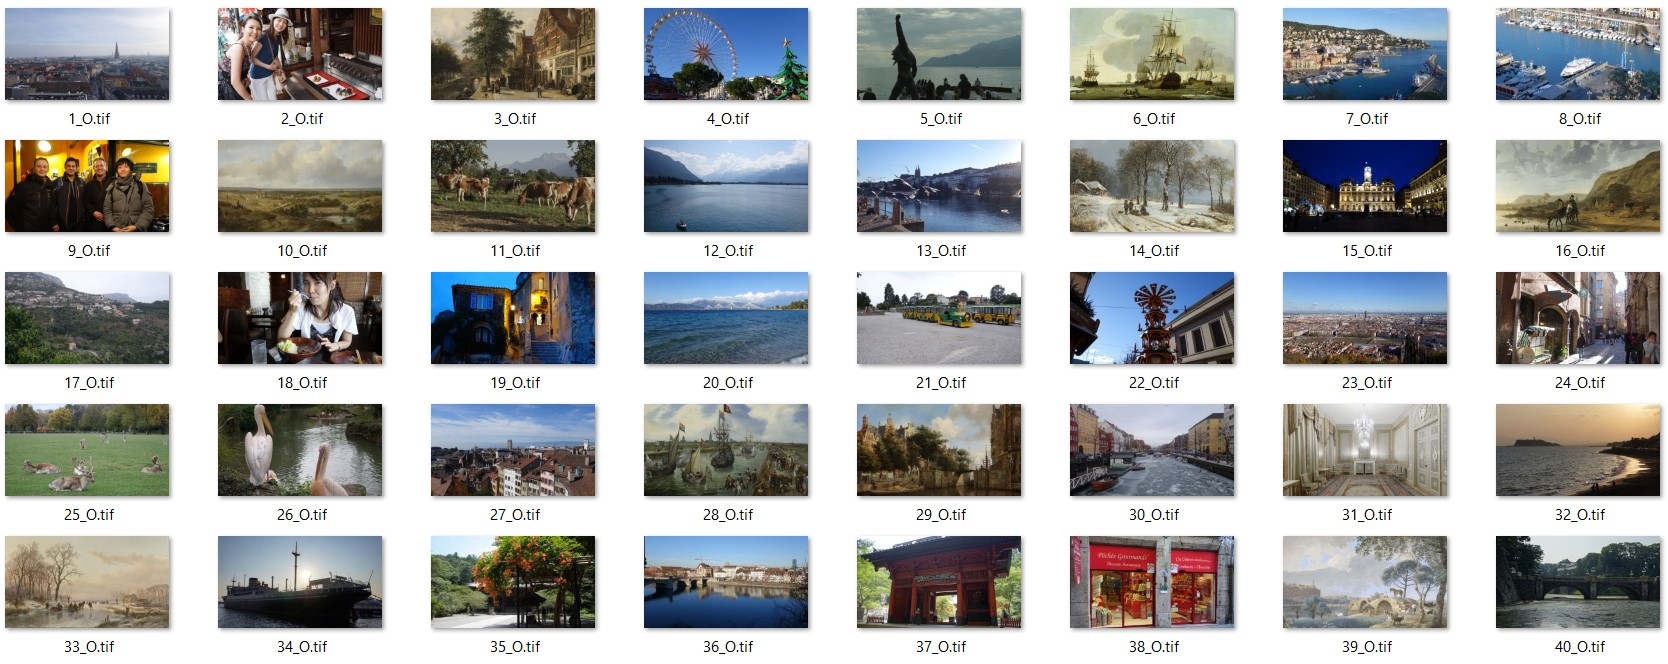
\includegraphics[scale=0.365]{dataset}
        \caption{"Dataset iniziale"}
    \end{figure}
    \\In particolare le elaborazioni sono state:
    \begin{enumerate}
        \item Per ogni immagine nel dataset iniziale è stata generata un'immagine in una risoluzione minore o uguale (4K, 3K, 2K, 1K, 720p, 480p) ed un'immagine compressa in JPEG con un livello di compressione variabile (0\%, 20\%, 40\%, 60\%, 80\%, 100\%);
        \item Per ogni immagine generata al punto 1 è stato applicato un filtro blur (sfocatura) su 8 intensità diverse.
    \end{enumerate}
    Questo procedimento ha così generato 3960 immagini, utilizzabili per addestrare e testare la rete.
    
    \newpage
    \begin{figure}[h]
        \centering
        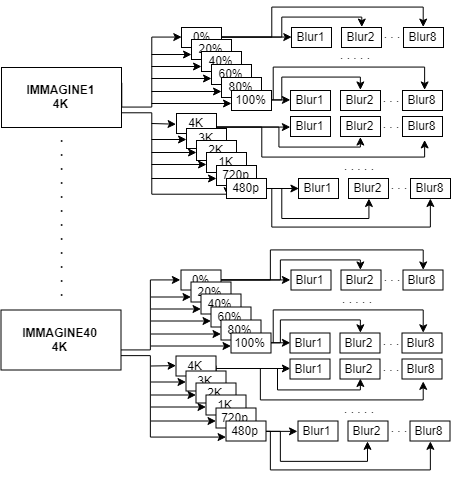
\includegraphics[scale=0.8]{generazione.png}
        \caption{"Generazione del dataset"}
    \end{figure}
    \newpage

    \subsubsection{Codice C++}
    Per ottenere il risultato precedentemente descritto è stato sviluppato un programma in C++ sfruttando la libreria OpenCV.
    Per ogni file nella directory delle immagini vengono prima generate le immagini compresse e le rispettive immagini filtrate:
    \begin{lstlisting}[language=C++]
    for (int i = 0; i <= 100; i += 20) {
			cout << "Compressing image " << fileName << " of " << i << "%" << endl;
			std::vector<int> params;
			params.push_back(CV_IMWRITE_JPEG_QUALITY);
			params.push_back(100 - i + i%100); 
			string format = (i==0) ? ".tif" : ".jpg";
			string newPath = basePath + "compressed/"+to_string(i)+"/" + fileName + format;

			if (i == 0)
				copyFile(filePath, newPath);
			else
				imwrite(newPath, imageOriginal, params);

			for (int intensity = 10; intensity <= 80; intensity += 10) {
				cout << "Blurring image " << fileName << " with intensity " << intensity << endl;
				Mat imageFiltered = applyFilter(newPath, "blur", intensity);
				string newPathFiltered = basePath + "compressed/" + to_string(i) + "/" + explode(fileName, '_')[0] + "_B" + to_string(intensity/10) + format;
				imwrite(newPathFiltered, imageFiltered);
			}
	}
    \end{lstlisting}
    \newpage
    Successivamente viene effettuato un procedimento simile per tutte le risoluzioni necessarie:
    \begin{lstlisting}[language=C++]
        for (dimension resolution : resolutions){
            cout << "Resizing image " << fileName << " to " << resolution.name << endl;
            Size size(resolution.height, resolution.width);
            Mat resizedImage;
            resize(imageOriginal, resizedImage, size);
            string newPath = basePath + "resized/" + resolution.name + "/" + fileName + ".tif";

            if (resolution.name.compare("4K") == 0) 
                copyFile(filePath, newPath);
            else
                imwrite(newPath, resizedImage);

            for (int intensity = 10; intensity <= 80; intensity += 10) {
                cout << "Blurring image " << fileName << " with intensity " << intensity << endl;
                Mat imageFiltered = applyFilter(newPath, "blur", intensity);
                string newPathFiltered = basePath + "resized/" + resolution.name + "/" + explode(fileName, '_')[0] + "_B" + to_string(intensity / 10) + ".tif";
                imwrite(newPathFiltered, imageFiltered);
            }
        }
    \end{lstlisting} 

    \newpage
    \subsubsection{Esempi}
    Di seguito vengono riportati alcuni esempi di immagini generate con il precedente procedimento le cui differenze sono facilmente percepibili ad occhio nudo.
    \begin{figure}[h]
        \centering
        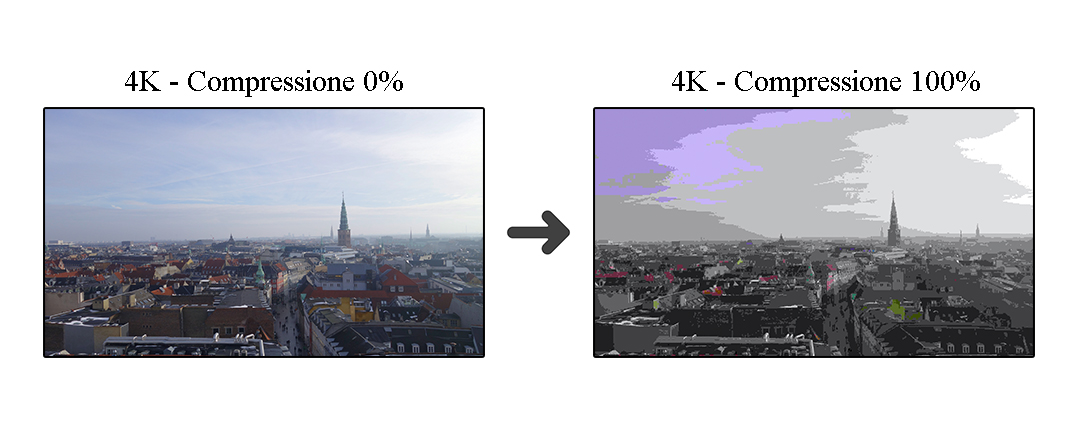
\includegraphics[scale=0.325]{compressione}
        \caption{"Esempio di compressione"}
    \end{figure}
    
    \begin{figure}[h]
        \centering
        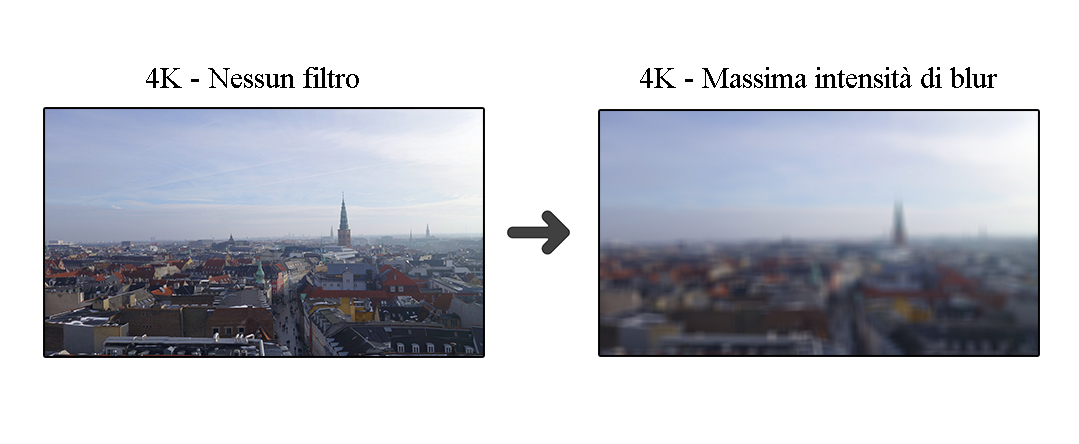
\includegraphics[scale=0.325]{blur}
        \caption{"Esempio di applicazione del filtro"}
    \end{figure}
    \subsubsection{Conversione nello spazio colore CIE L*a*b*}
    Le immagini del dataset sono inizialmente nello spazio RGB ma poiché si vuole cercare di simulare la percezione dell'occhio umano,
    si effettua la conversione nello spazio CIE L*a*b* utilizzando la libreria ImageMagick e convertendo tutte le immagini compresse con metodo JPEG in TIF, un formato capace di memorizzare immagini in questo spazio colore.
    \newpage

    \subsection{Addestramento della rete}
    \lipsum[1-3]

    \newpage
    \section{Test}
    \lipsum[1-3]

    \newpage
    \section{Conclusioni} 
    \lipsum[1-3]

    \newpage
    \section{Ringraziamenti}
    \lipsum[1-3]
    \end{document}
